% CVPR 2023 Paper Template
% based on the CVPR template provided by Ming-Ming Cheng (https://github.com/MCG-NKU/CVPR_Template)
% modified and extended by Stefan Roth (stefan.roth@NOSPAMtu-darmstadt.de)

\documentclass[10pt,twocolumn,letterpaper]{article}

%%%%%%%%% PAPER TYPE  - PLEASE UPDATE FOR FINAL VERSION
\usepackage{cvpr}      % To produce the REVIEW version

% Include other packages here, before hyperref.
\usepackage{graphicx}
\usepackage{amsmath}
\usepackage{amssymb}
\usepackage{booktabs}
\usepackage{subcaption}

% It is strongly recommended to use hyperref, especially for the review version.
% hyperref with option pagebackref eases the reviewers' job.
% Please disable hyperref *only* if you encounter grave issues, e.g. with the
% file validation for the camera-ready version.
%
% If you comment hyperref and then uncomment it, you should delete
% ReviewTempalte.aux before re-running LaTeX.
% (Or just hit 'q' on the first LaTeX run, let it finish, and you
%  should be clear).
\usepackage[pagebackref,breaklinks,colorlinks]{hyperref}

% Support for easy cross-referencing
\usepackage[capitalize]{cleveref}
\crefname{section}{Sec.}{Secs.}
\Crefname{section}{Section}{Sections}
\Crefname{table}{Table}{Tables}
\crefname{table}{Tab.}{Tabs.}

%%%%%%%%% PAPER ID  - PLEASE UPDATE
\def\cvprPaperID{*****} % *** Enter the CVPR Paper ID here
\def\confName{CVPR}
\def\confYear{2023}

\begin{document}

\newcommand{\dhimitrios}[1]{\textcolor{red}{Dhimitrios: #1}}

%%%%%%%%% TITLE - PLEASE UPDATE
\title{Team \#16: From Strings to Sequences --- Classifying and Generating Music from Acoustic Guitar Notes}


\author{
  Camilo Martínez\\
  7057573\\
  \and
  Dhimitrios Duka\\
  7059153\\
  \and
  Honglu Ma\\
  7055053\\
}
\maketitle

%%%%%%%%% BODY TEXT
\section{Abstract}
% Should be inside \emph{} https://openaccess.thecvf.com/content/CVPR2022W/WMF/papers/Guarnera_On_the_Exploitation_of_Deepfake_Model_Recognition_CVPRW_2022_paper.pdf
\emph{Lorem ipsum dolor sit amet, consectetur adipiscing elit}

\section{Introduction}

\section{Related Work}  

\section{Method}

\subsection{Datasets}
\dhimitrios{Not sure if Datasets should be under methods}

We identified a significant gap in available datasets for the task of guitar chord recognition, which made us create our own. We recorded 90-second videos for each chord in three different environments, ensuring high quality by capturing them in 4K resolution at 60 frames per second. From these videos, we extracted frames and downsampled them to a resolution of 640 $\times$ 360 pixels. This process generated approximately 30,000 frames per chord.

\begin{figure}[h]
  \centering
  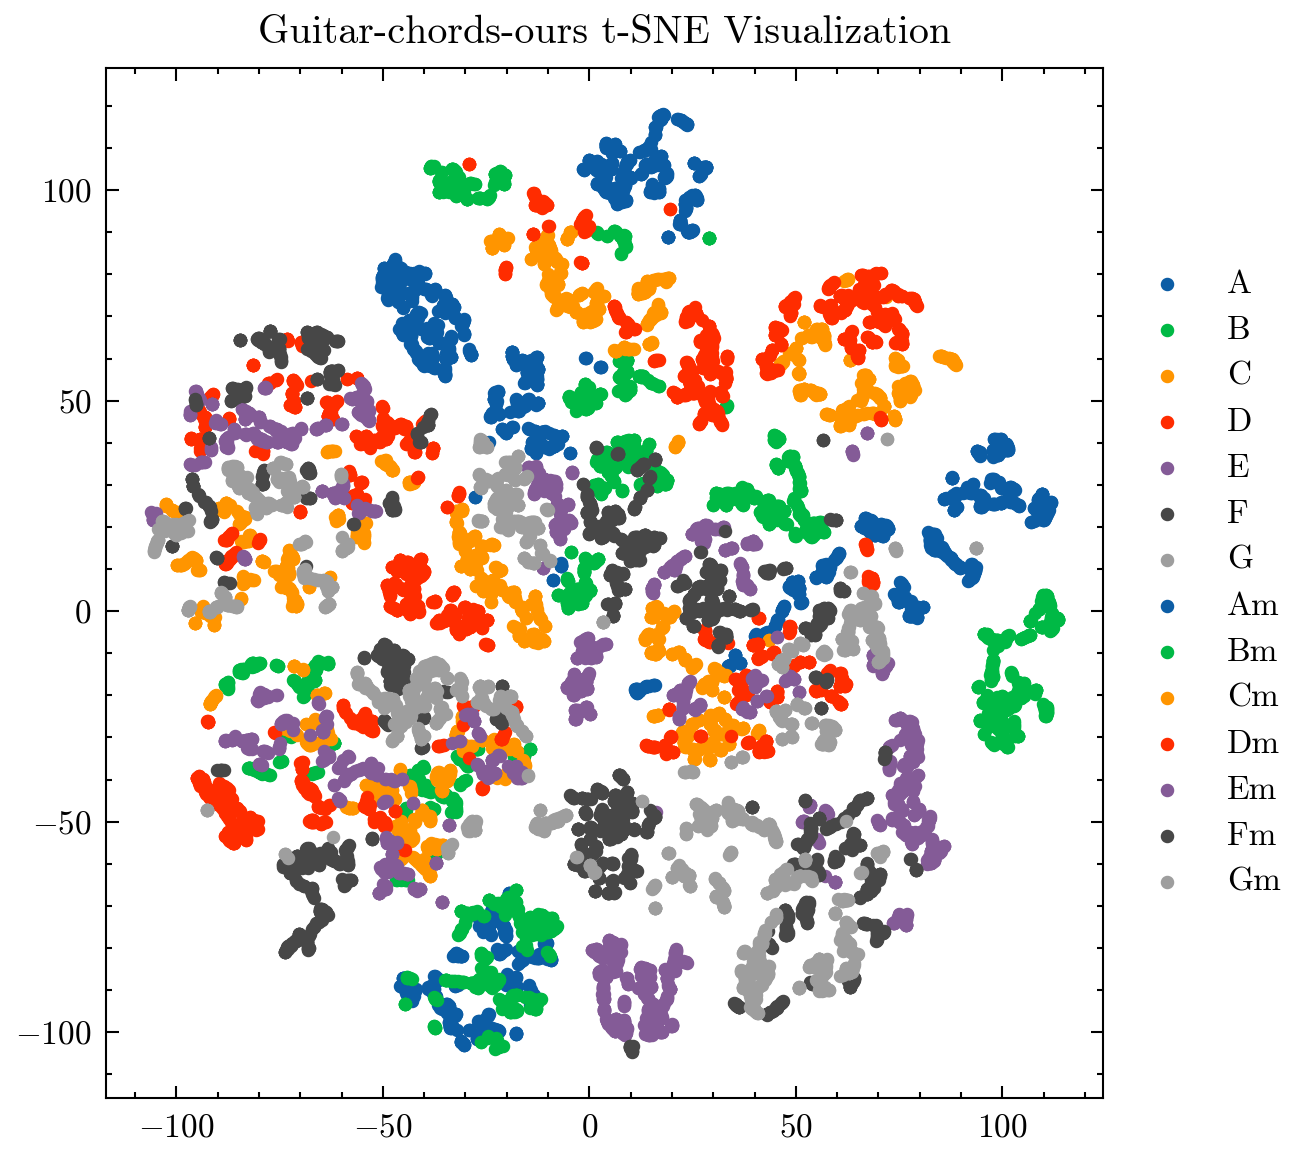
\includegraphics[width=0.3\textwidth]{images/final/Guitar-chords-ours_tsne_plot.png}
  \caption{t-SNE plot of our dataset. Each point represents a frame, and the color indicates the chord label. }
  \label{fig:ours-tsne-plot}
\end{figure}

To reduce redundancy, we limit the dataset to 1,000 frames for each of the 14 chords. To increase the diversity of the dataset, we used two different sampling methods: simple random sampling and KNN-based sampling. In the former method, we selected 1,000 frames at random. In the latter method, we used the KNN algorithm to choose 1,000 frames that were the most distinct from one another.

Unfortunately, both sampling strategies resulted in an overly simplistic dataset that failed to capture the real-world complexity of chords, as shown by Figure \ref{fig:ours-tsne-plot}. This resulted in poor model generalization. However, rather than abandoning our dataset named \textbf{Guitrar\_chords\_ours}, we used it as a test set to evaluate the generalizability of our model. In the end, we decided to use existing datasets \cite{guitar-chord-tvon8_dataset,guitar-chord-bounding-box_dataset, guitar-chord-handshape_dataset, guitar-chords-daewp_dataset} for training the models, merging them to create a more complex dataset named \textbf{Guitar\_chords}, which resulted in significantly better results.

\dhimitrios{Maybe I can also add something about augmentations here.}

\section{Experimental Results and Analyses}
\label{sec:results}

\subsection{Guitar Chord Classification}
To peform chord classfification we implemented different approaches, incluing Hand pose estimation + Classifier, a simple CNN like MobileNetV2 or InceptionResNetV2, and more complex architectures like ViT \cite{} and DINOv2 \cite{}.

\subsubsection{Hand Pose Estimation + Classifier}
First, we wanted to try a simple but interesting approache. The idea is simple. For each frame, we would use a hand pose estimation model to extract the hand shape and then use its output as the input to a classfifer. 

\begin{figure}[h]
  \centering
  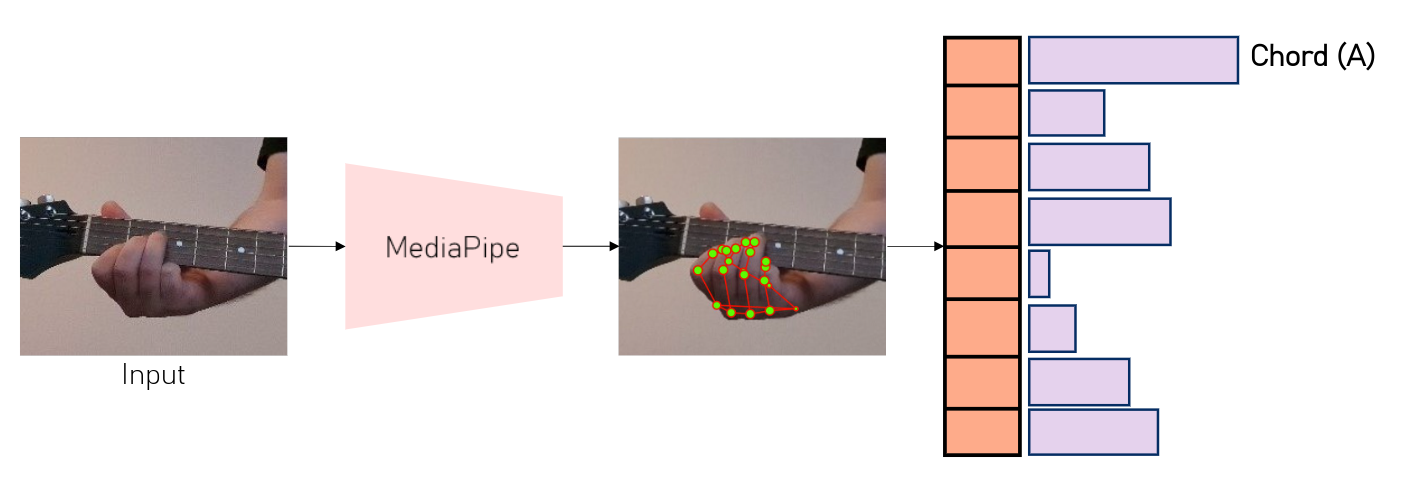
\includegraphics[width=0.5\textwidth]{images/final/hand_pose_estimation_classifier.png}
  \caption{t-SNE plot of our dataset. Each point represents a frame, and the color indicates the chord label. }
  \label{fig:ours-tsne-plot}
\end{figure}

We used the MediaPipe Handpose model \cite{} to extract the hand shape and then used different classifiers like SVM, Random Forest, and a simple MLP to classify the chords. Surprisingly, this approach worked well, achieving good accuracy during validation and testing with 2 out of three datasets. However, the model failed to generalize to the third dataset, which was the one we created. This was expected, as the samples in the dataset are out of distribution and the model is not complex enough to generalize to them. 

The results of this approach are shown in Table \ref{tab:handpose-classifier-results}.

\begin{table}[h]
  \centering
  \begin{tabular}{lccc}
    \toprule
    \textbf{Model} & \textbf{GC} & \textbf{GCT} & \textbf{GCO} \\
    \midrule
    SVM & 95.27\% & 85.71\% & 18.61\% \\
    Random Forest & 93.35\% & 52.41\% & 16.16\%  \\
    MLP & 89.44\% & 78.57\% & 14.39\% \\
    \bottomrule
  \end{tabular}
  \caption{Results of the Hand Pose Estimation + Classifier in different datasets. \textbf{GC}: Guitar\_Chords, \textbf{GCT}: Guitar\_Chords\_Tiny, \textbf{GCO}: Guitar\_Chords\_Ours.}
  \label{tab:handpose-classifier-results}
\end{table}

\section{Conclusion}

 %%%%%%%%% REFERENCES
 {\small
  \bibliographystyle{ieee_fullname}
  \bibliography{references}
 }

\end{document}